\documentclass[a4paper,12pt,oneside]{book}
\usepackage{polski}
\usepackage[utf8]{inputenc}
\usepackage{graphicx}
\graphicspath{{./images}}
\usepackage[shortlabels]{enumitem}
\usepackage{amssymb}
\usepackage{amsmath}
\usepackage{indentfirst}

\usepackage{tikz}
%\usepackage{etoolbox} % for \ifthen
\usepackage{listofitems} % for \readlist to create arrays
\usetikzlibrary{arrows.meta} % for arrow size
\usepackage[outline]{contour} % glow around text
\contourlength{1.4pt}

\tikzset{>=latex} % for LaTeX arrow head
\usepackage{xcolor}
\colorlet{myred}{red!80!black}
\colorlet{myblue}{blue!80!black}
\colorlet{mygreen}{green!60!black}
\colorlet{myorange}{orange!70!red!60!black}
\colorlet{mydarkred}{red!30!black}
\colorlet{mydarkblue}{blue!40!black}
\colorlet{mydarkgreen}{green!30!black}
\tikzstyle{node}=[thick,circle,draw=myblue,minimum size=22,inner sep=0.5,outer sep=0.6]
\tikzstyle{node in}=[node,green!20!black,draw=mygreen!30!black,fill=mygreen!25]
\tikzstyle{node hidden}=[node,blue!20!black,draw=myblue!30!black,fill=myblue!20]
\tikzstyle{node convol}=[node,orange!20!black,draw=myorange!30!black,fill=myorange!20]
\tikzstyle{node out}=[node,red!20!black,draw=myred!30!black,fill=myred!20]
\tikzstyle{connect}=[thick,mydarkblue] %,line cap=round
\tikzstyle{connect arrow}=[-{Latex[length=4,width=3.5]},thick,mydarkblue,shorten <=0.5,shorten >=1]
\tikzset{ % node styles, numbered for easy mapping with \nstyle
	node 1/.style={node in},
	node 2/.style={node hidden},
	node 3/.style={node out},
}
\def\nstyle{int(\lay<\Nnodlen?min(2,\lay):3)} % map layer number onto 1, 2, or 3

\def\shrug{\texttt{\raisebox{0.75em}{\char`\_}\char`\\\char`\_\kern-0.5ex(\kern-0.25ex\raisebox{0.25ex}{\rotatebox{45}{\raisebox{-.75ex}"\kern-1.5ex\rotatebox{-90})}}\kern-0.5ex)\kern-0.5ex\char`\_/\raisebox{0.75em}{\char`\_}}}

\renewcommand\thesubsection{\arabic{subsection}}
\renewcommand\thechapter{\Roman{chapter}}
\renewcommand\thesection{\arabic{section}}
\renewcommand\thesubsection{(\alph{subsection})}

\begin{document}

	\tableofcontents
	\newpage

	\chapter{Pytania - dr. hab. Bogdan Księżopolski}
		
		\setcounter{section}{65}
		\section{Charakterystyka kryptografii symetrycznej oraz asymetrycznej.}
		
		\subsection*{Kryptografia symetryczna}
				
			W kryptografii symetrycznej szyfrowanie i deszyfrowanie wykonywane jest przy użyciu tego samego klucza. W niektórych algorytmach wykorzystywane są dwa klucze, jednak muszą one być od siebie zależne w taki sposób, że znając jeden z nich, można wygenerować drugi.
			
			\begin{figure}[h!]
				\centering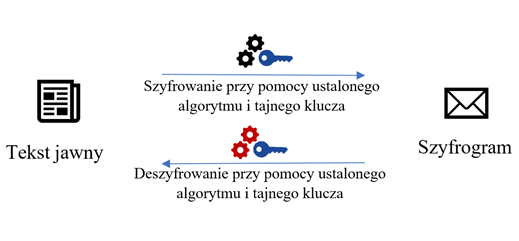
\includegraphics[scale=0.45]{krypt_sym.png}
				\caption{Zasada działania kryptografii symetrycznej}
			\end{figure}
			
			W celu zapewnienia bezpiecznej komunikacji, algorytm szyfrowania musi być tak skonstruowany, żeby odtworzenie tekstu jawnego bez znajomości klucza było zadaniem trudnym obliczeniowo. Dodatkowym wymaganiem jest tajność klucza – przed rozpoczęciem wymiany wiadomości, należy opracować protokół uzgadniania lub przekazywania klucza.
			
			Algorytmy szyfrowania symetrycznego możemy podzielić na algorytmy blokowe i strumieniowe. Pierwsze z nich przekształcają blok danych ustalonej długości, traktując go jako całość, na szyfrogram o tej samej liczbie bitów. Szyfry strumieniowe przyjmują natomiast ciąg (strumień) danych. Algorytmy kryptografii symetrycznej są szybkie, zwykle wymagają też mniejszej mocy obliczeniowej niż algorytmy asymetryczne. Powszechnie stosowanym szyfrem symetrycznych jest \textbf{AES}.
			
			\subsection*{Kryptografia asymetryczna}
			
			Kryptografia asymetryczna to rodzaj kryptografii, w którym jeden z używanych kluczy jest udostępniony publicznie. Każdy użytkownik może użyć tego klucza do zaszyfrowania wiadomości, ale tylko posiadacz drugiego, tajnego klucza może odszyfrować taką wiadomość.
			
			Kryptografia asymetryczna opiera się na funkcjach jednokierunkowych – takich, które da się łatwo wyliczyć w jedną stronę, ale bardzo trudno w drugą. Np. mnożenie jest łatwe, a rozkład na czynniki (z ang. faktoryzacja) trudny (na czym przykładowo opiera się \textbf{RSA}). Potęgowanie modulo jest łatwe, a logarytmowanie dyskretne jest trudne (na czym opierają się ElGamal, DSA i \textbf{ECC}).
			
			\begin{figure}[h]
				\centering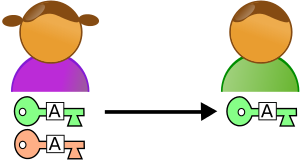
\includegraphics[scale=0.45]{krypt_asym_1.png}
				\caption{Krok 1: Alice przesyła do Boba swój klucz publiczny}
				
				\hspace{5pt}
				
				\centering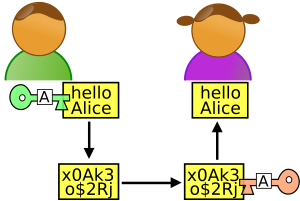
\includegraphics[scale=0.45]{krypt_asym_2.png}
				\caption{Kroki 2 i 3: Bob szyfruje wiadomość kluczem publicznym Alice, która to następnie otrzymuje zaszyfrowaną wiadomość i rozszyfrowuje ją kluczem prywatnym}
			\end{figure}
			
			Klucz publiczny używany jest do zaszyfrowania informacji, klucz prywatny do jej odczytu. Ponieważ klucz prywatny jest w wyłącznym posiadaniu adresata informacji, tylko on może ją odczytać. Natomiast klucz publiczny jest udostępniony każdemu, kto zechce zaszyfrować wiadomość.
			
			Ponieważ kryptografia asymetryczna jest o wiele wolniejsza od symetrycznej, prawie nigdy nie szyfruje się wiadomości za pomocą kryptosystemów asymetrycznych (również ze względu na ograniczenie wielkości szyfrowanej wiadomości). Zamiast tego szyfruje się jedynie klucz jakiegoś szyfru symetrycznego, takiego jak np. AES. Takie protokoły, łączące elementy kryptografii symetrycznej i asymetrycznej, nazywa się hybrydowymi.
			
			Nadawcy mogą także używać kluczy prywatnych do cyfrowego podpisywania wiadomości. Te podpisy cyfrowe pozwalają odbiorcom uwierzytelnić tożsamość nadawcy i spać spokojnie, wiedząc, że wiadomości nie zostały zmienione od momentu podpisania. W takim przypadku przesyłane informacje mogą być publiczne, a odbiorca może użyć certyfikatu, który towarzyszy tej informacji, aby zweryfikować integralność i autentyczność podpisanej wiadomości.
			
			\begin{figure}[h]
				\centering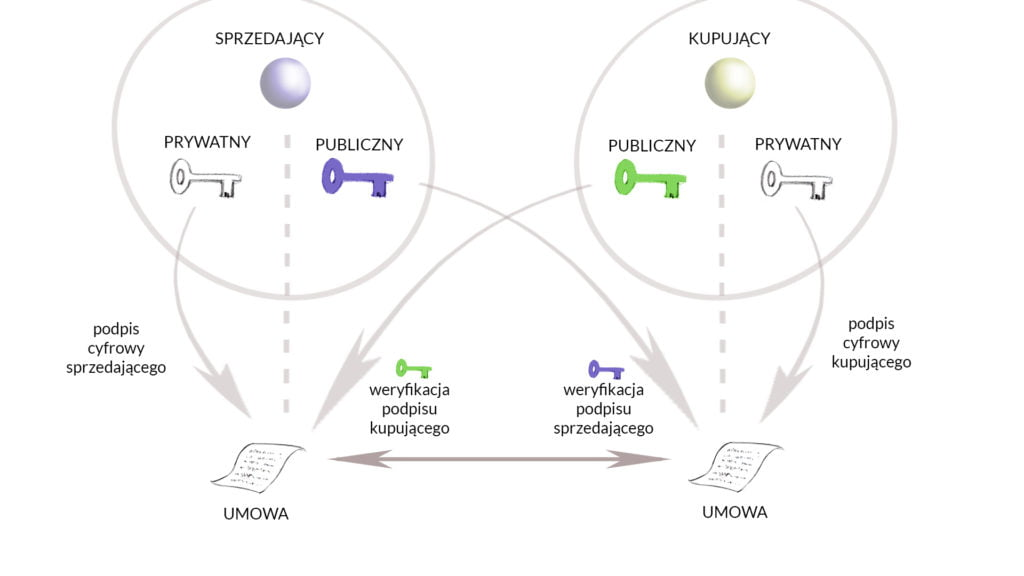
\includegraphics[scale=0.35]{krypt_asym_podpis.png}
				\caption{Jak działa podpis}
			\end{figure}
		
		\setcounter{section}{1}
		\section{Funkcje skrótu (mieszające) i ich zastosowania. }
		
			\addcontentsline{toc}{subsubection}{2. Funkcje skrótu (mieszające) i ich zastosowania}
			Funkcja skrótu, funkcja mieszająca lub funkcja haszująca – funkcja przyporządkowująca dowolnie dużej liczbie krótką wartość o stałym rozmiarze, tzw. skrót nieodwracalny.\\
			
			W informatyce funkcje skrótu pozwalają na ustalenie krótkich i łatwych do weryfikacji sygnatur dla dowolnie dużych zbiorów danych. Sygnatury mogą chronić przed przypadkowymi lub celowo wprowadzonymi modyfikacjami danych (sumy kontrolne), a także mają zastosowania przy optymalizacji dostępu do struktur danych w programach komputerowych (tablice mieszające).\\
			
			Szczególną podgrupą funkcji skrótu są funkcje uznawane za bezpieczne do zastosowań kryptologicznych (jak np. SHA-3). Kryptograficzna funkcja skrótu powinna spełniać kombinację następujących kryteriów, w zależności od zastosowania:\\
			\begin{itemize}
				\item Odporność na kolizje (collision resistance) – brak praktycznej możliwości wygenerowania dwóch dowolnych wiadomości o takim samym skrócie
				\item Odporność na kolizje konkretnych wiadomości (target collision-resistance, preimage resistance) pierwszego i drugiego rzędu – brak praktycznej możliwości wygenerowania wiadomości o takim samym skrócie jak wskazana wiadomość
				\item Jednokierunkowość (one-wayness) – brak możliwości wnioskowania o wiadomości wejściowej na podstawie wartości skrótu. Zmiana dowolnego pojedynczego bitu wiadomości powinna zmieniać średnio połowę bitów skrótu w sposób, który nie jest istotnie podatny na kryptoanalizę różnicową.
			\end{itemize}
			
			Przykładowe funkcje skrótu to SHA-1 (SHA128), SHA-2 (SHA256), SHA-3(SHA512), MD5.
		
		\setcounter{section}{8}
		\section{\color{red} TODO: Protokoły TCP i UDP – porównanie i zastosowanie.}
		
		Lorem ipsum dupa dupa
		
		\setcounter{section}{9}
		\section{\color{red} TODO: Adresowanie w warstwie Internetu modelu TCP/IP.}
		
		Lorem ipsum dupa dupa
		
		\setcounter{section}{11}
		\section{\color{red} TODO: Porównanie modelu OSI i TCP/IP. }
		
		Lorem ipsum dupa dupa
		
		\setcounter{section}{12}
		\section{\color{red} TODO: Mechanizm enkapsulacji w modelu OSI. }
		
		Lorem ipsum dupa dupa
		
		\setcounter{section}{57}
		\section{\color{red} TODO: Mechanizm sesji w zarządzaniu stanem aplikacji sieciowej. }
		
		Lorem ipsum dupa dupa
		
		\setcounter{section}{58}
		\section{\color{red} TODO: Mechanizm gniazd – pojęcie, sposób realizacji i zastosowanie }
		
		Lorem ipsum dupa dupa
		
		\setcounter{section}{59}
		\section{\color{red} TODO: Metody obsługi wielu klientów równolegle w aplikacjach sieciowych.}
		
		Lorem ipsum dupa dupa
		
		\setcounter{section}{60}
		\section{\color{red} TODO: Pocztowe protokoły warstwy aplikacji. }
		
		Lorem ipsum dupa dupa
		
		\setcounter{section}{61}
		\section{\color{red} TODO: Porównanie HTTP i WebSocket. }
		
		Lorem ipsum dupa dupa
		
		\setcounter{section}{62}
		\section{\color{red} TODO: Atrybuty bezpieczeństwa informacji. }
		
		Lorem ipsum dupa dupa
		
		\setcounter{section}{63}
		\section{\color{red} TODO: Modele dystrybucji kluczy kryptograficznych.}
		
		Lorem ipsum dupa dupa
		
		\setcounter{section}{64}
		\section{\color{red} TODO: Rodzaje zagrożeń oraz ochrona aplikacji sieciowych.}
		
		Lorem ipsum dupa dupa
		
		
	
	\chapter{Pytania - dr. hab. Grzegorz Wójcik}
		
		\setcounter{section}{32}
		\section{Budowa sieci neuronowych}
				
			\begin{figure}[h!]
						\centering
						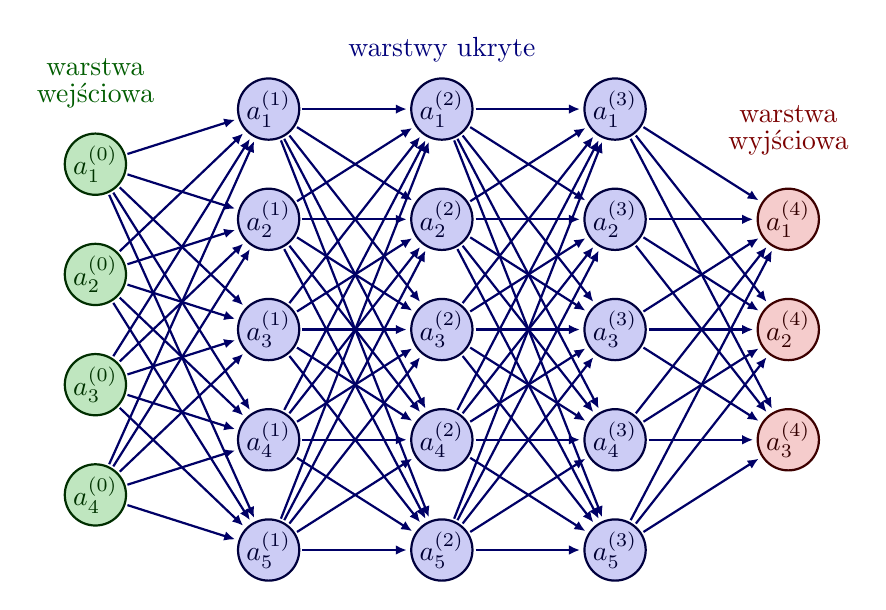
\begin{tikzpicture}[x=2.2cm,y=1.4cm]
							\message{^^JNeural network with arrows}
							\readlist\Nnod{4,5,5,5,3} % array of number of nodes per layer
							
							\message{^^J  Layer}
							\foreachitem \N \in \Nnod{ % loop over layers
								\edef\lay{\Ncnt} % alias of index of current layer
								\message{\lay,}
								\pgfmathsetmacro\prev{int(\Ncnt-1)} % number of previous layer
								\foreach \i [evaluate={\y=\N/2-\i; \x=\lay; \n=\nstyle;}] in {1,...,\N}{ % loop over nodes
									
									% NODES
									\node[node \n] (N\lay-\i) at (\x,\y) {$a_\i^{(\prev)}$};
									%\node[circle,inner sep=2] (N\lay-\i') at (\x-0.15,\y) {}; % shifted node
									%\draw[node] (N\lay-\i) circle (\R);
									
									% CONNECTIONS
									\ifnum\lay>1 % connect to previous layer
									\foreach \j in {1,...,\Nnod[\prev]}{ % loop over nodes in previous layer
										\draw[connect arrow] (N\prev-\j) -- (N\lay-\i); % connect arrows directly
										%\draw[connect arrow] (N\prev-\j) -- (N\lay-\i'); % connect arrows to shifted node
									}
									\fi % else: nothing to connect first layer
									
								}
								
							}
						
	  \node[above=5,align=center,mygreen!60!black] at (N1-1.90) {warstwa\\[-0.2em]wejściowa};
							\node[above=2,align=center,myblue!60!black] at (N3-1.90) {warstwy ukryte};
							\node[above=8,align=center,myred!60!black] at (N\Nnodlen-1.90) {warstwa\\[-0.2em]wyjściowa};
						\end{tikzpicture}
						\end{figure}
						
						Sieci neuronowe, znane również jako sztuczne sieci neuronowe lub symulowane sieci neuronowe są częścią funkcji uczenia maszynowego i stanowią podstawę algorytmów uczenia głębokiego. Ich nazwa i struktura są wzorowane na ludzkim mózgu i naśladują sposób, w jaki biologiczne neurony komunikują się między sobą.
						
						Sztuczne sieci neuronowe składają się z warstw węzłów, obejmujących warstwę wejściową, jedną lub więcej warstw ukrytych oraz warstwę wyjściową. Każdy węzeł (sztuczny neuron) łączy się z innym i ma powiązaną wagę oraz próg. Jeśli wyjście dowolnego pojedynczego węzła przekracza określoną wartość progową, węzeł ten jest aktywowany podczas wysyłania danych do kolejnej warstwy sieci. W przeciwnym razie żadne dane nie są przekazywane do następnej warstwy sieci.
						
						\begin{figure}[h!]
							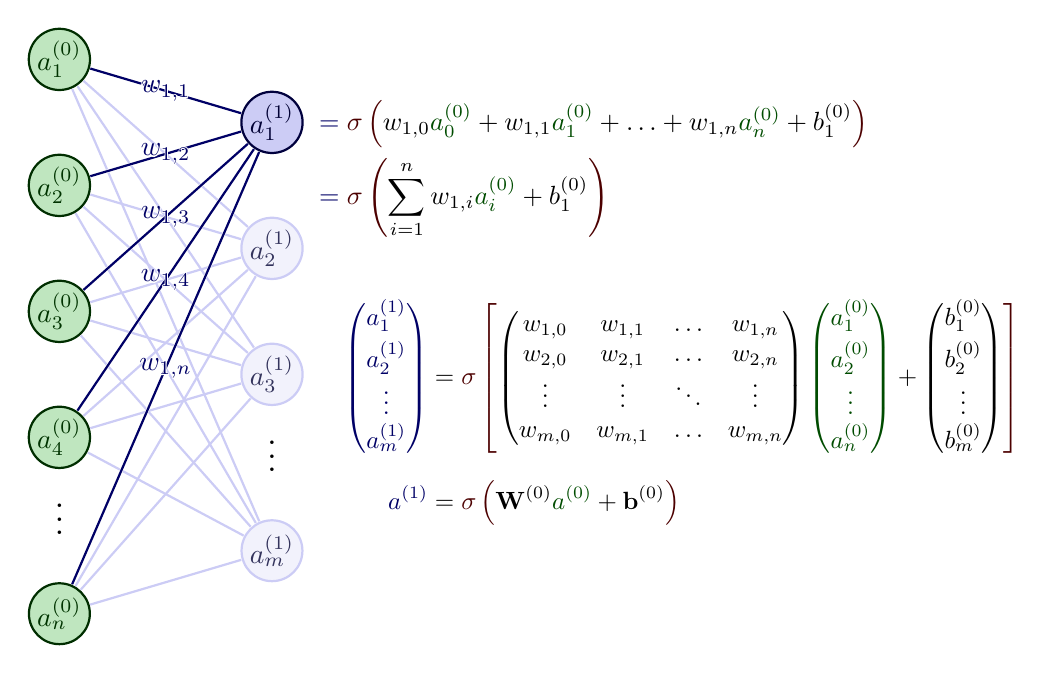
\begin{tikzpicture}[x=2.7cm,y=1.6cm]
								\message{^^JNeural network activation}
								\def\NI{5} % number of nodes in input layers
								\def\NO{4} % number of nodes in output layers
								\def\yshift{0.4} % shift last node for dots
								
								% INPUT LAYER
								\foreach \i [evaluate={\c=int(\i==\NI); \y=\NI/2-\i-\c*\yshift; \index=(\i<\NI?int(\i):"n");}]
								in {1,...,\NI}{ % loop over nodes
									\node[node in,outer sep=0.6] (NI-\i) at (0,\y) {$a_{\index}^{(0)}$};
								}
								
								% OUTPUT LAYER
								\foreach \i [evaluate={\c=int(\i==\NO); \y=\NO/2-\i-\c*\yshift; \index=(\i<\NO?int(\i):"m");}]
								in {\NO,...,1}{ % loop over nodes
									\ifnum\i=1 % high-lighted node
									\node[node hidden]
									(NO-\i) at (1,\y) {$a_{\index}^{(1)}$};
									\foreach \j [evaluate={\index=(\j<\NI?int(\j):"n");}] in {1,...,\NI}{ % loop over nodes in previous layer
										\draw[connect,white,line width=1.2] (NI-\j) -- (NO-\i);
										\draw[connect] (NI-\j) -- (NO-\i)
										node[pos=0.50] {\contour{white}{$w_{1,\index}$}};
									}
									\else % other light-colored nodes
									\node[node,blue!20!black!80,draw=myblue!20,fill=myblue!5]
									(NO-\i) at (1,\y) {$a_{\index}^{(1)}$};
									\foreach \j in {1,...,\NI}{ % loop over nodes in previous layer
										%\draw[connect,white,line width=1.2] (NI-\j) -- (NO-\i);
										\draw[connect,myblue!20] (NI-\j) -- (NO-\i);
									}
									\fi
								}
								
								% DOTS
								\path (NI-\NI) --++ (0,1+\yshift) node[midway,scale=1.2] {$\vdots$};
								\path (NO-\NO) --++ (0,1+\yshift) node[midway,scale=1.2] {$\vdots$};
								
								% EQUATIONS
								\def\agr#1{{\color{mydarkgreen}a_{#1}^{(0)}}}
								\node[below=17,right=11,mydarkblue,scale=0.95] at (NO-1)
								{$\begin{aligned} %\underset{\text{bias}}{b_1}
										&= \color{mydarkred}\sigma\left( \color{black}
										w_{1,0}\agr{0} + w_{1,1}\agr{1} + \ldots + w_{1,n}\agr{n} + b_1^{(0)}
										\color{mydarkred}\right)\\
										&= \color{mydarkred}\sigma\left( \color{black}
										\sum_{i=1}^{n} w_{1,i}\agr{i} + b_1^{(0)}
										\color{mydarkred}\right)
									\end{aligned}$};
								\node[right,scale=0.9] at (1.3,-1.3)
								{$\begin{aligned}
										{\color{mydarkblue}
											\begin{pmatrix}
												a_{1}^{(1)} \\[0.3em]
												a_{2}^{(1)} \\
												\vdots \\
												a_{m}^{(1)}
										\end{pmatrix}}
										&=
										\color{mydarkred}\sigma\left[ \color{black}
										\begin{pmatrix}
											w_{1,0} & w_{1,1} & \ldots & w_{1,n} \\
											w_{2,0} & w_{2,1} & \ldots & w_{2,n} \\
											\vdots  & \vdots  & \ddots & \vdots  \\
											w_{m,0} & w_{m,1} & \ldots & w_{m,n}
										\end{pmatrix}
										{\color{mydarkgreen}
											\begin{pmatrix}
												a_{1}^{(0)} \\[0.3em]
												a_{2}^{(0)} \\
												\vdots \\
												a_{n}^{(0)}
										\end{pmatrix}}
										+
										\begin{pmatrix}
											b_{1}^{(0)} \\[0.3em]
											b_{2}^{(0)} \\
											\vdots \\
											b_{m}^{(0)}
										\end{pmatrix}
										\color{mydarkred}\right]\\[0.5em]
										{\color{mydarkblue}a^{(1)}}
										&= \color{mydarkred}\sigma\left( \color{black}
										\mathbf{W}^{(0)} {\color{mydarkgreen}a^{(0)}}+\mathbf{b}^{(0)}
										\color{mydarkred}\right)
										%\color{black},\quad \mathbf{W}^{(0)} \in \mathbb{R}^{m\times n}
									\end{aligned}$};
								
							\end{tikzpicture}
						\end{figure}
						
						O każdym pojedynczym węźle należy myśleć jak o modelu regresji liniowej złożonym z danych wejściowych, wag, odchyleń (lub wartości progowych) i danych wyjściowych. Rysunek powyżej przedstawia właśnie te obliczenia dla jednego neurona. Macierz $\mathbf{W}^{(0)}$ jest macierzą wszystkich wag wchodzących do każdego neurona warstwy $a^{(0)}$ z warstwy poprzedniej, wektor $b^(0)$ to wartości wszystkich \textit{bias-ów} danej warstwy, a $\sigma$ to funkcja aktywacji danej warstwy.
						
						Wagi pomagają określić znaczenie każdej zmiennej, przy czym większe z nich mają większy wpływ na wynik wyjściowy w porównaniu do innych danych wejściowych. Wszystkie dane wejściowe są następnie mnożone przez swoje odpowiednie wagi, a potem sumowane. Następnie wyniki są przepuszczane przez funkcję aktywacji, która określa wartość wyjściową.
		
		\setcounter{section}{29}
		\section{\color{red} TODO: Modele reprezentacji wiedzy.}
				
				Lorem ipsum dupa dupa
		
		\setcounter{section}{30}
		\section{\color{red} TODO: Mechanizmy wnioskowań. }
				
				Lorem ipsum dupa dupa
		
		\setcounter{section}{31}
		\section{\color{red} TODO: Metody uczenia maszynowego.} 
				
				Lorem ipsum dupa dupa
		
		\setcounter{section}{33}
		\section{\color{red} TODO: Normalizacja baz danych – pierwsza, druga i trzecia postać normalna. }
				
				Lorem ipsum dupa dupa
		
		\setcounter{section}{34}
		\section{\color{green}Paweł \color{red} TODO: Modele baz danych (logiczny, relacyjny, fizyczny). }
				
				Lorem ipsum dupa dupa
		
		\setcounter{section}{35}
		\section{\color{green}Paweł \color{red} TODO: Rodzaje zapytań w języku SQL. }
				
				Lorem ipsum dupa dupa
		
		\setcounter{section}{36}
		\section{\color{green}Paweł \color{red} TODO: Funkcje w języku SQL. }
				
				Lorem ipsum dupa dupa
		
		\setcounter{section}{37}
		\section{\color{green}Paweł \color{red} TODO: Transakcje w bazach danych.} 
				
				Lorem ipsum dupa dupa
		
		
		\setcounter{section}{14}
		\section{\color{red} TODO: Hermetyzacja, dziedziczenie i polimorfizm w programowaniu obiektowym. }
				
				Lorem ipsum dupa dupa
				
		\setcounter{section}{47}
		\section{\color{red} TODO: Główne paradygmaty programowania – charakterystyka i przykłady. }
						
				Lorem ipsum dupa dupa
				
		\setcounter{section}{16}
		\section{\color{red} TODO: Paradygmat i przykłady programowania generycznego (rodzajowego). }
								
						Lorem ipsum dupa dupa
	
	\chapter{Pytania - reszta}
		
		\setcounter{section}{0}
		\section{Wektory i macierze – definicje i podstawowe operacje.}
				
			Macierz to układ liczb, symboli lub wyrażeń zapisanych w postaci prostokątnej tablicy. W algebrze liniowej macierze wprowadza się często jako sposób skondensowanego zapisu układów równań liniowych, co ma na celu wyeliminowanie powtarzających się elementów standardowej notacji układów równań tego rodzaju z wieloma niewiadomymi. Macierze pozwalają również na reprezentowanie przekształceń liniowych w sposób umożliwiający przeprowadzanie obliczeń. Ponieważ wiele przekształceń geometrycznych (jak na przykład obroty przestrzeni $\mathbb {R} ^{n}$ wokół początku układu współrzędnych) są przekształceniami liniowymi, macierze znajdują zastosowanie w geometrii analitycznej i grafice komputerowej.
			
			Przykład zapisu macierzy $3\times 3$
			$ \begin{bmatrix}
				8 & 3 & 2 \\
				5 & 4 & 1 \\
				2 & 9 & 0 
			\end{bmatrix}  $
			
			Macierze ${\displaystyle \mathbf {A} =[a_{ij}]}$ i ${\displaystyle \mathbf {B} =[b_{ij}]}$ uważa się za równe, jeśli mają ten sam typ i równe odpowiadające sobie elementy, tzn. dla każdej możliwej pary $i,j$ zachodzi ${\displaystyle a_{ij}=b_{ij}.}$\\
			
			Sumę macierzy $\mathbf{A}$ i $\mathbf{B}$ definiuje się „po współczynnikach”, tzn. za pomocą wzoru $\mathbf {A+B} =[a_{ij}+b_{ij}]$ dla wszystkich $i,j.$ Z definicji wynika (ale można napisać wprost), że można dodawać macierzy tylko o takich samych wymiarach.
			
			\begin{center}
				$ \begin{bmatrix}
					8 & 3 & 2 \\
					5 & 4 & 1 \\
					2 & 9 & 0 
				\end{bmatrix} + 
			\begin{bmatrix}
				2 & 2 & 6 \\
				3 & 5 & 7 \\
				1 & 0 & 4 
			\end{bmatrix} = 
		\begin{bmatrix}
			10 & 5 & 8 \\
			8 & 10 & 8 \\
			3 & 9 & 4 
		\end{bmatrix}$
			\end{center}
			
			Mnożenie przez skalar macierzy $\mathbf{A}$ oraz liczby $c$ również definiuje się „po współczynnikach”, czyli $c\mathbf {A} =[ca_{ij}]$ dla dowolnych $ i,j.$\\
			\begin{center}
				$ 2 * \begin{bmatrix}
					8 & 3 & 2 \\
					5 & 4 & 1 \\
					2 & 9 & 0 
				\end{bmatrix} = 
			\begin{bmatrix}
				16 & 6 & 4 \\
				10 & 8 & 2 \\
				4 & 18 & 0 
			\end{bmatrix}$
			\end{center}
		
			Działanie mnożenia macierzy jest zdefiniowane najczęściej jako tzw. iloczyn Cauchy'ego: dla dla macierzy ${\mathbf  A}$ typu $m\times n$ oraz $\mathbf{B}$ typu $n \times p$ dany jest on jako taka macierz $\mathbf C$ typu $m\times p,$ oznaczana $\mathbf {AB} ,$ dla której
			
			$c_{ij}=a_{i1}b_{1j}+a_{i2}b_{2j}+\dots +a_{in}b_{nj}$ dla dowolnych $i,j.$\\
			
			Mnożenie to jest łączne ($A(BC)=(AB)C$), ale nie jest przemienne ($AB \neq BA$).\\
			
				\begin{center}
				$\begin{bmatrix}
					2 & 3 & 7 \\
					6 & 1 & 2 
				\end{bmatrix} 
				\begin{bmatrix}
					1 \\
					0\\
					5 
				\end{bmatrix} = 
				\begin{bmatrix}
				2 * 1 + 3 * 0 + 7 * 5\\
				6 * 1 + 1 * 0 + 2 * 5
			\end{bmatrix}=
			\begin{bmatrix}
				37\\
				16
			\end{bmatrix}$
			\end{center}
			
			
			
			\begin{figure}[h!]
				\centering
				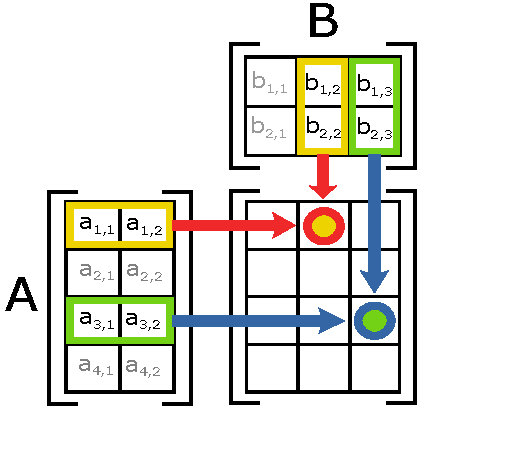
\includegraphics[scale=0.8]{Matrix_multiplication_diagram_2.pdf}
				\caption{Schemat mnożenia macierzy A i B}
			\end{figure}
		
			Elementem neutralnym mnożenia macierzy przez siebie jest macierz diagonalna, zawierająca na swojej przekątnej same jedynki.
					\begin{center}
				$\begin{bmatrix}
					2 & 3 & 7 \\
					6 & 1 & 2 
				\end{bmatrix} 
				\begin{bmatrix}
					1 & 0 & 0 \\
					0 & 1 & 0\\
					0 & 0 & 1 
				\end{bmatrix} = 
				\begin{bmatrix}
					2 & 3 & 7 \\
					6 & 1 & 2 
				\end{bmatrix}$ 
			\end{center}
		
			Przestawienie bądź transpozycja danej macierzy $\mathbf {A}$, tzn. zamiana jej kolumn i wierszy miejscami (z zachowaniem kolejności). Macierz transponowaną lub przestawioną względem macierzy $\mathbf  A$ definiuje się jako macierz
			
			$\mathbf {A} ^{\mathrm {T} }=[a_{ji}]$ dla wszystkich $i,j,$ przy czym $(\mathbf {AB} )^{\mathrm {T} }=\mathbf {B} ^{\mathrm {T} }\mathbf {A} ^{\mathrm {T} }$ oraz $\left(\mathbf {A} ^{\mathrm {T} }\right)^{\mathrm {T} }=\mathbf {A} .$\\
			
			Wyznacznikiem $\det(\mathbf {A} )$ lub $|\mathbf {A} |$ macierzy kwadratowej $\mathbf  A$ nazywa się liczbę kodującą pewne właściwości przekształcenia $\mathrm {A}$ reprezentowanego przez tę macierz. \\
			
			Wyznacznik macierzy stopnia drugiego dany jest wzorem
			\begin{center}
					${\displaystyle \det {\begin{bmatrix}a&b\\c&d\end{bmatrix}}=ad-bc.}$\\
			\end{center}
		
			
			
			Wektor jest macierzą o wymiarach $n\times 1$. Reprezentuje on punkt w przestrzeni $\mathbb{R}^n$. Jego podstawowe trzy cechy to:
			\begin{itemize}
				\item długość - czasami inaczej zwana modułem lub wartością
				\item kierunek - kierunek prostej zawierającej wektor
				\item zwrot - grot strzałki
			\end{itemize}
		
			\begin{figure}[h!]
				\centering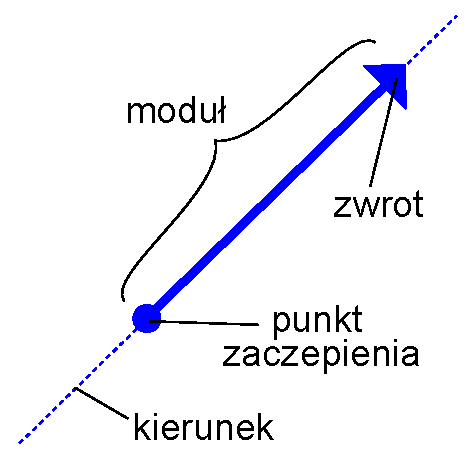
\includegraphics[scale=0.7]{Wektor_by_Zureks.pdf}
				\caption{Ilustracja wektora}
			\end{figure}
		
			Dodawanie oraz mnożenie przez skalar wektora jest zdefiniowane w ten sam sposób jak w przypadku macierzy. \\\\\\
			
			
			Iloczyn skalarny dwóch wektorów to \textbf{liczba}, którą obliczamy dodając iloczyny odpowiednich współrzędnych.
			
			\begin{center}
				$\vec{a}=[2,1,3], \vec{b}=[4,1,2]$\\
				$\vec{a}\circ\vec{b} = 2*4 + 1*1 + 3*2 = 15$
			\end{center}
		
			Iloczyn skalarny możemy również obliczyć znając długości wektorów $|\vec{a}|$ i $|\vec{b}|$ oraz kąt $\alpha$ między nimi:
			
			\begin{center}
				$\vec{a}\circ\vec{b}=\|\vec{a}\|*\|\vec{b}\|*\cos\alpha$
			\end{center}
		
			Długość wektora $\vec{a}$ może być zdefiniowana jako pierwiastek iloczynu skalarnego z samym sobą. 
			
			\begin{center}
				$\|\vec{a}\|=\sqrt{\vec{a}\circ\vec{a}}$
			\end{center}
		
		Iloczyn wektorowy - działanie dwuargumentowe przyporządkowujące parze wektorów przestrzeni $\mathbb{R}^3$ pewien wektor tej przestrzeni.\\
		
		Iloczyn wektorowy $\mathbf {a} \times \mathbf {b}$ wektorów $\mathbf a $ i $ \mathbf  b$ określa się następująco:
		\begin{itemize}
			\item jeśli wektory $\mathbf{a}$ i $\mathbf{b}$ są liniowo zależne, to $\mathbf{a}\times\mathbf{b}=0$
			\item jeśli wektory $\mathbf{a}$ i $\mathbf{b}$ nie są liniowo zależne, to $\mathbf{a}\times\mathbf{b}=\mathbf{c}$, gdzie $\mathbf{c}$ jest wektorem prostopadłym do płaszczyzny wyznaczonej przez $\mathbf{a}$ i $\mathbf{b}$.
		\end{itemize}
		
		\setcounter{section}{5}
		\section{Sposoby cyfrowej reprezentacji liczby całkowitej i rzeczywistej.}
				
			\subsubsection{Liczby całkowite}
			
			\subparagraph{Kod \text{ZM} (kod znak-moduł)}
			
			Sprawa w kodzie ZM jest w miarę prosta i klarowna. Najstarszy bit $b_{n-1}$ dla n-bitowej liczby jest bitem znaku i określa czy liczba jest dodatnia czy ujemna:
			\begin{itemize}
				\item 0 - liczba dodatnia,
				\item 1 - liczba ujemna.
			\end{itemize}
			
			Bity od $b_{n-1}$ do $b_0$ odpowiadają za kodowanie wartości samej liczby. Wzór na obliczenie wartości liczby zakodowanej w \textbf{ZM}:
			\begin{center}
				$L_{ZM} = (-1)^{b_{n-1}} \cdot (b_{n-2}2^{n-2} + ... + b_22^2 + b_12^1 + b_02^0)$
			\end{center}
			
			Przykładowe kodowanie liczby na ośmiu bitach w kodzie \textbf{ZM}:
			\begin{center}
				$26 \longrightarrow \textbf{0}0011010 $\\
				$-26 \longrightarrow \textbf{1}0011010 $
			\end{center}
			
			Proste, logiczne, fajne. Pytania, problemy? To jedziemy dalej.
			
				
			\subparagraph{Kod \textbf{U2} (kod uzupełnień do 2)}
			
			Tutaj sprawa się nieco komplikuje z zapisem liczb ujemnych. Bit $b_{n-1}$ ma wagę $-2^{n-1}$ co sprawia, że musimy bitowo tak jakby zapisać odwrotność liczby, którą chcemy reprezentować jako ujemna (i dodać 1, żeby się wszystko zgadzało). W zapisie liczb dodatnich zapis jest identyczny jak w \textbf{ZM} - na najstarszym bicie musimy tylko zachować $0$.
			
			Istnieje prosty algorytm konwersji na U2 z wykorzystaniem ZM:
			\begin{enumerate}
				\item Zapisać moduł liczby w ZM,
				\item Dokonać inwersji bitów (0 na 1 i 1 na 0),
				\item Zwiększ wynik dodając 1.
			\end{enumerate}
			
			Przykład z liczbą -27 na 8 bitach:
			
			\begin{tikzpicture}[x=2.2cm,y=1.4cm]
				\node[text width=5cm] at (0, 0)   (a) {Zapisujemy liczbę 27 w ZM};
				\node[text width=3cm] at (0.5, 1)   (b) {$00011011$};
				\draw [-to] (0,0.2) -- (0.2,0.7);
				\node[text width=3cm] at (2, 1)   (b) {$11100100$};
				\node[text width=3cm] at (3.5, 1)   (b) {$\textbf{11100101}$};
				
				\draw [-to] (0.7,1) -- (1.2,1);
				\draw [-to] (2.2,1) -- (2.7,1);
				
				\node[text width=5cm] at (2, 2)   (a) {Odwracamy bity};
				\draw [-to] (1.7,1.8) -- (1.7,1.2);
				
				\node[text width=5cm] at (3.9, 0)   (a) {Dodajemy 1};
				\draw [-to] (3.2,0.2) -- (3.2,0.7);
			\end{tikzpicture}
			
			\subsubsection{Liczby rzeczywiste}
			
			\subparagraph{Zapis stałopozycyjny}
			
			Do zapisu liczby stałoprzecinkowej przeznaczona jest z góry określona liczba bitów, a pozycję przecinka ustala się
			arbitralnie, w zależności od wymaganej dokładności, wolne bity uzupełniając zerami. Do reprezentacji liczb ze
			znakiem stosuje także kod U2.
			
			Liczba $6,25=110,01_{(2)}$ zapisana na 8 bitach gdy częśd ułamkowa zajmuje 3 najmłodsze bity, ma postać:
			\begin{center}
				\begin{tikzpicture}[x=2.2cm,y=1.4cm]	
					\node[text width=3cm] at (0, 0)   (b) {$\underbrace{00110}_{\text{część całkowita}}$};
					\node[text width=3cm] at (0.39, 0.42)   (b) {$\overbrace{010}^{\text{część ułamkowa}}$};
				\end{tikzpicture}
			\end{center}
			
			A w reprezentacji U2 będzie miała postać:
			
			\begin{center}
				$11001110$
			\end{center}
			
			Część całkowita liczby zachowuje się identycznie jak w przypadku zwykłych liczb całkowitych, natomiast bity w części ułamkowej posiadają wagi $2^{-1}$, $2^{-2}$, itd. - czyli $\frac{1}{2}$, $\frac{1}{4}$, ..., więc ilość bitów w części ułamkowej wpływa na precyzję zapisu.
			
			\subparagraph{Zapis zmiennopozycyjny}
			
			Liczba zmiennoprzecinkowa jest komputerową reprezentacją liczb rzeczywistych zapisanych w postaci wykładniczej
			o podstawie 2. Przykładowa notacja:
			
			\begin{center}
				$(-1)^Z \cdot M \cdot 2^C = (-1)^Z \cdot (1+m) \cdot 2^{c - BIAS}$
			\end{center}
			gdzie:
			\begin{description}
				\item[$(-1)^Z$] - znak liczby
				\item[$M=1+m$] - znormalizowana mantysa (liczba spełniająca warunek: $1 \leq M \leq 2$). Ponieważ przed przecinkiem stoi zawsze 1, więc można ją przedstawić w postaci $1+m$, gdzie \emph{m} jest liczbę ułamkową: $0 \leq m \leq 1$)
				\item[$C=c-BIAS$] - cecha (liczba całkowita), która dzięki zastosowaniu stałej BIAS pozwoli przedstawid cechę w postaci
				różnicy c-BIAS (c jest liczbą całkowitą dodatnią, tzw spolaryzowana cechę)
				\item[$BIAS$] - stała (liczba całkowita BIAS zależna od danej implementacji – rozwiązuje problem znaku cechy)
			\end{description}
			Kodujemy wyłącznie:
			\begin{description}
				\item[z] - bit znaku
				\item[m] - mantysę pomniejszoną o 1
				\item[c] - cechę przesuniętą o BIAS
			\end{description}
			
			Załóżmy, że operujemy następującym zmiennopozycyjnym formatem zapisu liczby rzeczywistej:
			\begin{itemize}
				\item na zapis przeznaczamy 16 bitów
				\item najstarszy bit ($b_{15}$) to bit znaku (będziemy stosowad kod ZM)
				\item kolejne 6 bitów ($b_{9}$-$b_{14}$) to mantysa
				\item pozostałe bity ($b_0$-$b_8$) są przeznaczone na zapis cechy i przyjmijmy, że BIAS=9
			\end{itemize}
			
			Przedstawimy liczbę +0,0224609375 w powyższym formacie. Naszą liczbę zapisujemy w systemie binarnym w
			postaci wykładniczej o podstawie 2, przesuwamy przecinek zapisując ją w notacji wykładniczej:
			
			\begin{center}
				$0,0224609375 = 0,0000010111_{(2)} = 1,0111_{(2)} \cdot 2^{-6}$
			\end{center}
			
			Z tego wynika, że:
			
			\begin{itemize}
				\item Znak: $(-1)^0$
				\item Mantysa: $1.\textbf{\underline{0111}}_2$
				\item Cecha: $-6 = 3-9 = 11_2 - BIAS$
			\end{itemize}
			
			Oto liczba 0,0224609375 zapisana w zadanym formacie:
			\begin{center}
				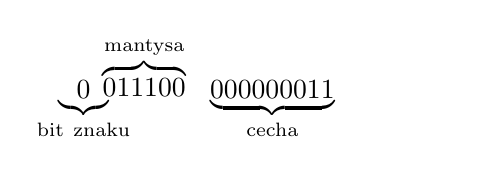
\begin{tikzpicture}[x=2.2cm,y=1.4cm]	
					\node[text width=3cm] at (0, 0)   (b) {$\underbrace{0}_{\text{bit znaku}}$};
					\node[text width=3cm] at (0.38, 0.39)   (b) {$\overbrace{011100}^{\text{mantysa}}$};
					\node[text width=3cm] at (1, 0)   (b) {$\underbrace{000000011}_{\text{cecha}}$};
				\end{tikzpicture}
			\end{center}
		
		\setcounter{section}{52}
		\section{Deklaratywne programowanie w logice: klauzule Horne'a, nawracanie.}
				
			Logika Hoare’a – formalizm matematyczny służący do opisu poprawności algorytmów.
			Trójka $\{P\}C\{Q\}$ oznacza, że fragment kodu $C$, o ile na wejściu będzie miał stan spełniający warunek $P$, oraz zakończy swoje działanie, to na wyjściu da stan spełniający warunek $Q$. Formułę $P$ nazywamy warunkiem wstępnym, a formułę $Q$ nazywamy warunkiem końcowym.\\
			
			Przykład:
			do instrukcji przypisania $x:=5$ możemy dopisać następujące warunki wstępne i końcowe:
				\begin{center}
						$\{{\text{true}}\}x:=5\{x=5\}$
				\end{center}
			co oznacza, że przy dowolnym stanie przed wykonaniem instrukcji, po wykonaniu instrukcji będziemy mieli stan, w którym zmiennej $x$ jest przypisana wartość 5.\\
			
			
			Prawdą jest też bardziej skomplikowana formuła:\\
			
			\begin{center}
				$\{x=y+z\}\{$if $x<y$ then $ z:=-z\}\{x\leq y+z\}$
			\end{center}
				
		\setcounter{section}{2}
		\section{\color{red} TODO: Problemy rekurencyjne i ich rozwiązywanie. }
		    
		    Lorem ipsum dupa dupa
		
		\setcounter{section}{4}
		\section{\color{red} TODO: Pozycyjne systemy liczbowe i konwersje pomiędzy nimi. }
		    
		    Lorem ipsum dupa dupa
		
		\setcounter{section}{6}
		\section{\color{red} TODO: Typ, zmienna, obiekt i zarządzanie pamięcią. }
		    
		    Lorem ipsum dupa dupa
		
		\setcounter{section}{7}
		\section{\color{green}Paweł \color{red} TODO: Instrukcje sterujące przepływem programu. }
		    
		    Lorem ipsum dupa dupa
		
		\setcounter{section}{10}
		\section{\color{red} TODO: Porównanie zadań przełącznika (switcha) i routera. }
		    
		    Lorem ipsum dupa dupa
		
		\setcounter{section}{13}
		\section{\color{red} TODO: Obiekt i klasa w wybranym języku programowania zorientowanym obiektowo. }
		    
		    Lorem ipsum dupa dupa
		
		\setcounter{section}{15}
		\section{\color{red} TODO: Interfejsy i klasy abstrakcyjne w programowaniu obiektowym. }
		    
		    Lorem ipsum dupa dupa
		
		\setcounter{section}{17}
		\section{\color{red} TODO: Algorytmy sortowania. }
		    
		    Lorem ipsum dupa dupa
		
		
		\setcounter{section}{18}
		\section{\color{red} TODO: Strategia „dziel i zwyciężaj” budowania algorytmów. }
		    
		    Lorem ipsum dupa dupa
		
		\setcounter{section}{19}
		\section{\color{red} TODO: Algorytmy typu zachłannego. }
		    
		    Lorem ipsum dupa dupa
		
		\setcounter{section}{20}
		\section{\color{red} TODO: Algorytmy z nawrotami. }
		    
		    Lorem ipsum dupa dupa
		
		\setcounter{section}{21}
		\section{\color{red} TODO: Grafy, drzewa, kopce – charakterystyka i przykłady zastosowania. }
		    
		    Lorem ipsum dupa dupa
		
		\setcounter{section}{46}
		\section{\color{green}Paweł \color{red} TODO: Definicja i klasy złożoności obliczeniowej – czasowej i pamięciowej. }
		    
		    Lorem ipsum dupa dupa
		
		\setcounter{section}{55}
		\section{Kodowanie liczb ze znakiem w systemie U2, generowanie liczby ze znakiem przeciwnym, dodawanie i odejmowanie. }
		
		    Patrz pytanie nr6 sposoby cyfrowej reprezentacji liczby całkowitej i rzeczywistej
		
	\chapter{Pytania których raczej nie dostaniemy}
	
	\setcounter{section}{27}
	\section{\color{red} TODO: Różnice pomiędzy obsługą zdarzeń w przerwaniach sprzętowych a obsługą zdarzeń w pętli programowej.}
					
					Lorem ipsum dupa dupa
	
	\setcounter{section}{28}
	\section{\color{red} TODO: Powody i przykłady stosowania mikrokontrolerów zamiast typowych komputerów. }
					
					Lorem ipsum dupa dupa
	
	\setcounter{section}{38}
	\section{\color{red} TODO: Standardowe metodyki procesu wytwórczego oprogramowania. }
					
					Lorem ipsum dupa dupa
	
	\setcounter{section}{39}
	\section{\color{red} TODO: Metodyki zwinne – SCRUM. }
					
					Lorem ipsum dupa dupa
	
	\setcounter{section}{40}
	\section{\color{red} TODO: Testowanie oprogramowania. }
					
					Lorem ipsum dupa dupa
	
	\setcounter{section}{41}
	\section{\color{red} TODO: Diagramy UML. }
					
					Lorem ipsum dupa dupa
	
	\setcounter{section}{42}
	\section{\color{red} TODO:  Wzorce projektowe programowania obiektowego. }
					
					Lorem ipsum dupa dupa
	
	\setcounter{section}{43}
	\section{\color{red} TODO: Definicja funkcji obliczalnej (częściowo rekurencyjnej). }
					
					Lorem ipsum dupa dupa
	
	\setcounter{section}{44}
	\section{\color{red} TODO: Maszyna Turinga jako model procesów obliczalnych. }
					
					Lorem ipsum dupa dupa
	
	\setcounter{section}{45}
	\section{\color{red} TODO: Zagadnienia nierostrzygalne w kontekście obliczalności. }
					
					Lorem ipsum dupa dupa
	
	\setcounter{section}{48}
	\section{\color{red} TODO:  Gramatyki bezkontekstowe – definicje, charakterystyki i przykłady. }
					
					Lorem ipsum dupa dupa
	
	\setcounter{section}{49}
	\section{\color{red} TODO: Analiza leksykalna, syntaktyczna i semantyczna kodu. }
					
					Lorem ipsum dupa dupa
	
	\setcounter{section}{50}
	\section{\color{red} TODO: Rodzaje błędów w kontekście analizy leksykalnej, syntaktycznej i semantycznej kodu.}
					
					Lorem ipsum dupa dupa
					
	\setcounter{section}{51}
	\section{\color{red} TODO: Deklaratywne programowanie funkcyjne: rachunek lambda, monady. }
					
					Lorem ipsum dupa dupa
	
	\setcounter{section}{53}
	\section{\color{red} TODO: Podstawowe układy systemu mikroprocesorowego i sposób wymiany informacji pomiędzy nimi. }
					
					Lorem ipsum dupa dupa
	
	\setcounter{section}{54}
	\section{\color{red} TODO: Dekoder, multiplekser i demultiplekser: budowa, zasada, działania, przeznaczenie, zastosowanie. }
					
					Lorem ipsum dupa dupa
	
	\setcounter{section}{56}
	\section{\color{red} TODO: Budowa i zasada działania generatora obrazu w systemie mikroprocesorowym. }
					
					Lorem ipsum dupa dupa
	
	\setcounter{section}{22}
	\section{\color{red} TODO: Wielowarstwowa organizacja systemów komputerowych. }
						
						Lorem ipsum dupa dupa
	
	\setcounter{section}{23}
	\section{\color{red} TODO: System operacyjny – charakterystyka, zadania, klasyfikacja. }
						
						Lorem ipsum dupa dupa
	
	\setcounter{section}{24}
	\section{\color{red} TODO: Procesy i wątki – charakterystyka i problemy. }
						
						Lorem ipsum dupa dupa
	
	\setcounter{section}{25}
	\section{\color{red} TODO: Zarządzanie pamięcią operacyjną w systemie operacyjnym. }
						
						Lorem ipsum dupa dupa
	
	\setcounter{section}{26}
	\section{\color{red} TODO: Organizacja systemu plików i pamięci zewnętrznej. }
						
						Lorem ipsum dupa dupa
						
	\setcounter{section}{2}
	\section{\color{red} TODO: Podstawowe charakterystyki statystyki opisowej i matematycznej.}
							
							Lorem ipsum dupa dupa
	
	
	
	
\end{document}